\documentclass[twocolumn]{revtex4}
\usepackage{graphics,graphicx,epsfig,amsmath,multirow,gensymb,commath,textcomp,natbib,blindtext,mhchem,tabularx,array,makecell}
\usepackage[a4paper, left=1.85cm, right=1.85cm, top=1.85cm, bottom=1.85cm]{geometry}   
\usepackage[normalem]{ulem}
\newcommand{\squeezeup}{\vspace{-2.5mm}}

\def\bibsection{\section*{\refname}} 
\renewcommand{\thesubsection}{\alph{subsection}}

\renewcommand\theadalign{bc}
\renewcommand\theadfont{\bfseries}
\renewcommand\theadgape{\Gape[4pt]}
\renewcommand\cellgape{\Gape[4pt]}

\begin{document}

\textheight=26.385cm
%Change textheight as the last resort...

\title{Producing light curves for Type Ia supernova explosions and exploring their uncertainties}
 
\author{Jacky Cao, AstroLabs Michaelmas, Lab Partner: Duncan Middlemiss \\ Dates of experiment: 19/10/2017 to 17/03/2017, Date of report: 19/03/2017}

\begin{abstract}              
We have measured the magnitude of supernova explosions over an extended period of 47 days using $0.5$ m and $?.?$ m telescopes situated in Durham and La Palma. We have plotted several light curves and identified Type Ia, Type II, and ?? supernovae. Our fittings have had $\chi^2$ analysis has performed, and it has produced values of ?, ?, ?. We expect our biggest source of uncertainty arose due to the conditions and data analysis that we performed. Using a Type Ia supernova of brightness $00.00$ mag, we have managed to produce a value for Hubble's Constant, $H_0 = 74$ kms$^{-1}$ Mpc$^{-1}$. We attempted to calculate Einstein's coefficient, $\Lambda$, but this was unsuccesful due to redsjhift of something.
\end{abstract}

\maketitle

\vspace{-3ex}
\section{Introduction} 
\label{intro}
\vspace{-2ex}

In astronomy, one of the most violent and luminous events which can occur are supernova explosions. At the end of a massive star's lifetime, there is a possibility that the equilibrium configurations for a star will cease to exist after it has ran out of nuclear fuel to burn. This leads to a final awesome event, a supernova explosion, the luminosity of which (when at it's peak) can be as bright as a small galaxy \cite{longair}.

Observing these events and measuring their magnitude over a period of time allows us to then plot light curves. The likes of which can then be used to visualise the evolution of a supernova, from this we can draw the conclusion that there is some order in the explosions. We find that if our sample of supernovae is large enough [find a value?], we see that they can be grouped together into different types just by features from their light curves, for example their shape.

\vspace{-3ex}
\subsection{Supernovae Classification}
\vspace{-2ex}

However, as we study the different spectra and light curve shapes of supernovae we begin to recognise that there are further sub-classifications \cite{longair}. Table \ref{sn_classes} highlights some of these subtypes. 

\begin{table}[h!]
\centering
\begin{tabular}{c@{\hskip 20pt}c} 
 \hline
 \textbf{Type} & \textbf{Characteristic} \\ 
 Type Ia		& Si II line at $616.0$ nm \\
 			& \em Type Ib and Type Ic also exist \em \\
 Type IIP 		& Reaches a plateau in it's light curve \\
 Type IIL		& Displays a linear decrease in it's light curve \\
 			& \em Type IIn and Type IIb also exist \em \\
 \hline
\end{tabular}
\caption{Some of the subclassifications of supernova \cite{longair}.}
\label{sn_classes}
\end{table}

In the application to cosmology one of the most used types of supernovae are Type Ia, their light curve profiles are generally homogenous which allows them to be effectively used as standard candles, thus providing another distance measure in the universe. With this we could work out the geometry of the universe by calculating the cosmological parameters, Hubble's Constant ($H_0$), and the proportion of the universe that is dark matter ($\Omega_{\Lambda}$). 

In Figure \ref{typeia-standard} we can see from multiple observation data, the light curves in B and V bands are generally homogenous. it must be noted that this graph which has been produced from archival supernova data, the actual magnitude peak at maximum brightness occurs at different days in different colour bands. More shall be explored of this in section [[whatever]].
\begin{figure}[!h]
\begin{center}
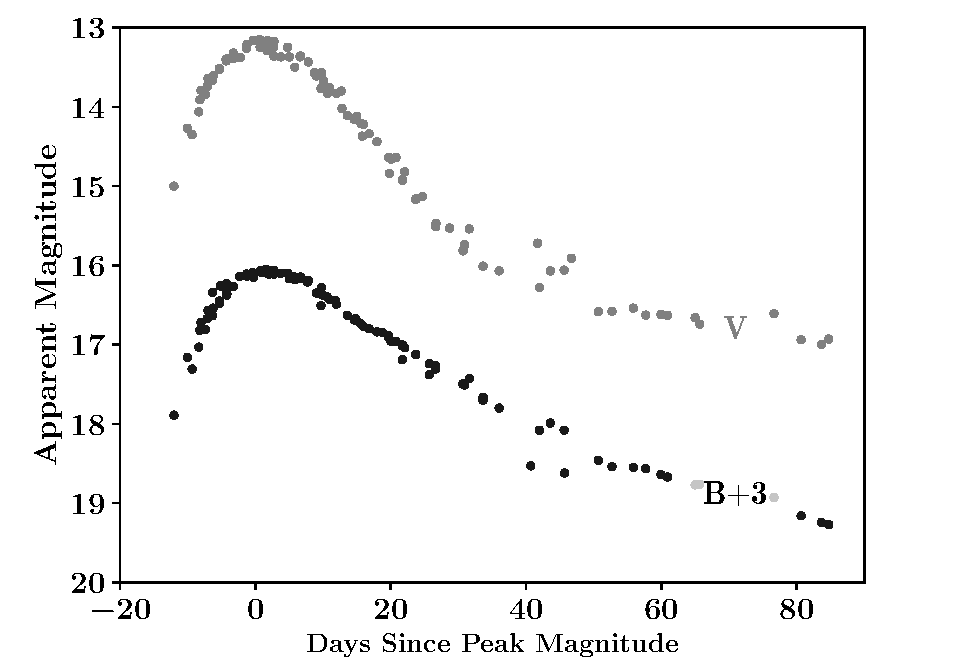
\includegraphics[width=9.5cm]{intro/typeia}
\caption[]{Plot showing the general forms of Type Ia supernovae in the B and V bands. The supernovae used are: \em{1994ae, 1994S, 1995bd, 1996bo, }\em  and \em{1998aq }\em \cite{jha, matheson}.}
\label{typeia-standard}
\end{center}
\end{figure}

\vspace{-3ex}
\subsubsection{Type I Supernovae}
\vspace{-2ex}
In understanding why the optical spectra of Type I supernovae do not contain the Balmer hydrogen features, we must look at the physical composition of the objects. Type I SNe occur with stars which have lost their hydrogen envelopes, either from strong mass-loss from their surface layers, or because they involve the explosion of white dwarfs which lost their hydrogen envelopes when they were formed \cite{longair} [[does that make sense??]]. 

With the important of Type Ia supernovae as distance moduli we will explore the systems that lead up to their explosion, the explosion mechanism, and what occurs post explosion.

The general consensus for the presupernova of Type Ia supernovae, there is a white dwarf within a binary system which accretes matter from a donor star. However, this is also the initial system for dwarf novae and classical novae, better known together as cataclysmic variables \cite{mod_ast}. They too increase in brightness which can lead to some confusion with supernovae, especially if you observe them initially optically. If observed spectroscopically we could potentially determine whether it is a supernova and which type as we would be able to identify which elements are present [[not sure about this]]. With classical novae as they increase in their brightness by a factor of  $\sim 10^6$ \cite{mod_ast}. [more detail??]

The distinction for supernovae is drawn as the white dwarf will increase in it's mass until it reaches the critical Chandrasekhar mass, $1.4 M_{\odot}$ \cite{posn, longair}. As the material is continually compressed on and in the white dwarf, it is heated to a temperature of $T \geq 10^9$ K \cite{longair}, the fusion of the rich carbon and oxygen core can begin. Thermonuclear energy is released and the white dwarf loses it's electron degeneracy pressure, the object is now gravitationally unstable \cite{longair}. However, this energy that is produced disrupts the star and prevents a total collapse into a neutron star, this disruption leads to a supernova explosion \cite{posn}. 

This white dwarf-comapnion star mechanism has support from spectroscopic observations of Type Ia supernovae at maximum light. We find the spectra has silicon, calcium, magnesium, sulphur and oxygen present. These are elements which are the products for when carbon and oxygen are burned in the nuclear fusion processes of (\ce{^{12}C} + \ce{^{12}C}), and (\ce{^{16}O} + \ce{^{16}O}) \cite{longair}.

From spectral fits, we can calculate the velocities of the ejecta material which have been measured to have a range from a mean value of $5,000$ kms$^{-1}$, to a peak that exceeds $20,000$ kms$^{-1}$ \cite{ia_vel}, approximately $7\%$ of the speed of light. Supernovae are incredibly energetic events with the majority of the explosion energy being converted into kinetic \cite{posn}, these explosions offer us a chance to calculate some fundamental properties of the universe [???].

As this process relies on the Chandrasekhar limit, each Type Ia supernova which occurs will be the same as they would follow the same process of collapsing. They are useful as they  

When plotting their magnitudes against time passed we see that their light curves are generally homogeneous. These objects are the most luminous supernovae known, their absolute magnitudes in the B band are typically $M_B = -19.5 \pm 0.1$ \cite{posn}. Using light curve relationships and models we can determine precisely the magnitudes of very distant SNe, this has allowed astronomers to determine the redshift-distance relation for redshifts high redshift objects ($z>1$). Then, with these calculated values it is then possible to estimate the cosmological parameters $\Omega_0$ and $\Omega_\Lambda$. In doing so, it has been found that using Type Ia SNe has produced agreement with the literature value. so and so (cite paper) have done this and produced values of. 

\vspace{-3ex}
\subsubsection{Type II Supernovae}
\vspace{-2ex}
Somehow retie in Type II, it's not as important as Type Ia for our experiment but it should suffice to be mentioned!

For a star to end it's life as a Type II supernova explosion, it's core must collapse to produce the enormous amounts of energy that we associate with a SNe. For stars more massive than $8 M_{\odot}$, their post-main-sequence evolution relies on the continual burning of carbon, oxygen, and silicon burning. As this process continues to heat up the core to larger temperatures, photodisintegration will start to occur. Photons have enough energy to breakup heavier elements such as iron (\ce{^{56}_{26}Fe}) and helium (\ce{^{4}_{2}He}), this process is endothermic so energy is removed from the gas that would have created the pressure required to support the core of the star \cite{mod_ast}. 

The free electrons which had been supporting the star through degeneracy pressure are now captured by heavy nuclei and by the protons that were produced through photodisintegration. Through the photodisintegration of iron, and combined with electron capture by other elements, most of the core's support disappears and then the core begins to collapse extremely rapidly. 

\vspace{-3ex}
\subsection{Supernova Discovery}
\vspace{-2ex}
In discovering supernovae it is important that the search is not focussed on a singular part of the sky as there is a possibility that they could occur in any region of the sky. What is required is a survey which covers the entire visible sky. Then, the general method that is employed is that each night's data can be compared on a day-to-day basis and any new objects that appear could be classified as a supernovae. Follow up observations are required though to verify if it actually is a new object exploding or whether it is an anomalous object such as a cataclysmic variable. [reference] 

One such survey that employs this is the \em{All-Sky Automated Survey for Supernovae }\em (or ASAS-SN). Their setup (??) involves two stations based in Halekala Observatory in Hawaii, and Cerro Tololo International Observatory in Chile. Together they can produce a survey of the entire visible sky up to a depth of $\sim 17$ mag \cite{asn_lc}.

With this case specifically it has been set so that the data is taken automatically, but it requires humans to go over it. Another method that can be used is to observe a location such as a galactic cluster and do essentially the same method.

In the classification of supernovae and in determining their redshifts, spectroscopic observations are required on the objects after they have been discovered \cite{lascumbres}. While we can use light curves to find the type of a supernova, it is more effective to use their spectra as that will allow us to be more certain [??].

\vspace{-3ex}
\subsection{Application to Cosmology} \label{appcosmo}
\vspace{-2ex}
In discovering supernovae we can calculate the rates at which supernovae occur. Surveying different parts of the sky we can produce an estimate for the rate at which supernova explosions happen.



asdasd \cite{abs_phil}
\begin{equation}
v = H_0 d, 
\end{equation}
with $v$ as the velocity of the receding object, $H_0$ as the value for Hubble's 
find a reference for this.

\vspace{-3ex}
\subsection{Project Aims}
\vspace{-2ex}
This paper outlines the study that was undertaken in an attempt to understand the evolution of the magnitudes of different supernovae over a time period [[?]]. From collected data it would be possible to produce light curves which we can use to identify the type of supernova that we were observing. In also understanding the uncertainties further analysis could be performed such as galaxy subtraction or [[think of something for here...]].

Section \ref{obsver} describes the methods used to collect and analyse the data, plus the uncertainties that arise during the experiment and how they were dealt with. Our final light curves, and the methods that were used to fit these models to the observations is summarised in Section \ref{analysis}. Section \ref{discussion} discusses the different blahj blah blah, and explores potential work that could be performed. With Section \ref{conclusions} provididng a summary and conlusion.

We also focussed on understanding the sources of uncertainties and attempted to reduce them within our analysis to produce magnitudes which would be more true to what they should be [[?]]. 

\vspace{-3ex}
\section{Observations} 
\label{obsver}
\vspace{-2ex}
\subsection{Data Collection}
\vspace{-2ex}

Observing supernova explosions requires instruments which are sensitive enough to receive the photons which have travelled for vast distances before being recorded. In performing such observations (?) our main equipment are telescopes - they come in a wide variety of configurations and each can produce different results.

In collecting the data for our supernova we used three different types of telescopes. Two of them based in Durham on the Department of Physic's Roof, and one in La Palma. 

As we were observing objects which were faint we required that we either have a large telescope to collect as much light as possible [reference], or have good seeing conditions which allowed us to collect as much light as possible over a large observation time.

In performing our observations, Far-East-16 and pt5m (give basic broad descriptions of these telescopes - tell how they are big and thus how much light they can collect?) was used. 

Talk about the CCDs, their specs, and what that implies. Any uncertainties work should be either stated here, or in the uncertainties section, or spoken about in both. 

Reliant on weather conditions being acceptable to observe in, define acceptable, discuss clouds, seeing, atmospheric turbulence, Lumiere, temperature, ...etc

in observations how has the moon affected us


\vspace{-3ex}
\subsection{Observations Made}
\vspace{-2ex}

Over a period of (?) days we took images of SNe, however this also depended on the conditions and whether it was worth observing if the seeing was bad e.g. obscured by bad weather.

In making observations there were various factors which required to be known.

In Appendix \ref{objectslog} is detailed all the objects that we chose to view over our experimental period, and in Appendix \ref{obslogs} is a more detailed description of the data that we took.

\vspace{-3ex}
\subsection{Data Analysis}
\vspace{-2ex}

[[WHAT TENSE AM I SUPPOSED TO USE? PAST OR PRESENT??]]

As we collected our supernova data over our experimental period we were then required to perform various photometry techniques to calculate the magnitudes of the explosions. It is important that this method was correct as we wanted accurate representations of the light curves. 

With our \em{raw}\em data we firstly needed to identify our supernoa object, as these objects can blend in with the background of stars we had to look it up for the right ascenscion and declination reference. All of our supernova objects were discovered by other astronomers so they had an initial set of information we could use like, astronomical location on the celestial sphere, initial magnitude and the discovery date.

Once we had found our object we needed to find the magnitude of it. Using an astronomical analysis package such as GAIA [[reference and improve this]], we used various tools to perform this. We had to understand that we wanted to find the absolute mangitude of the supernoiva, this value being the 'actual magnitude', and not relative to other objects [[?]]. To perform this we had to choose at least two calibration stars which have known absolute magnitiudes.

To count the number of counts that we are receiving from our supernova and calibration objects we have to choose an apperture size to place over these objects. It is important thatthe radius that is chosen maximises the signal whilst reducing the amount of noise that we are receving as well, it is important that we have the cleanest signal possible.

To do this an object was selected which was close to the supernova and appeared to be similar in size, this was normally one of the calibration stars that we would be using. With our software package [[and for astronomy?]] we also had to choose a size for the 'sky aperture', this was so that the sky noise could be removed from the counts as well. In choosing this we had to account for the proximity of the supernova to its host galaxy's nucleus and also on how close the calibration stars are to other stars. We did not want to include unessecary data that would produce an errorneous result. 

After a sky aperture had been chosen we would then try and find the best radius to use when doing our photometry. This radius would be constant for our calibration objects and for our supernova as well, and also for each day's data frames. This would ensure that we would be not 'cherrypicking' the signal that we are receving and that it would be an 'equal opportunity' for the signal to be detected to be the same each time [[??]]. 

This radius would be chosen by adjusting it from one to twenty in integer steps of one, noting down number of counts, the uncertainty on that value, and the sky noise counts. After these values had been collected we would plot the signal to noise against radius. In the plot, where the graph reaches a peak and decreases after this pooint would be our radius size as this would be the radius where we would achieve maximum signal to noise.

Then we can collect the values for the counts of the supernova and calibration objects, once we have this data we can use equation \ref{mag_counts} to find the absolute magnitude of the supernova. [[give a reference for the equation from a paper]]

\begin{equation}
    m = z - 2.5 \log_{10}{C},
\label{mag_counts}
\end{equation}

where $m$ is the absolute magnitude that we are trying to find, $z$ is the 'zero-point' of our frame [[is it how much it's offset by??]], and $C$ is the number of counts we receive from our object.

In using this equation we must have the correct zero-point, $z$, otherwise we would not be finding the absolute magnitude, instead the apparent magnitude relative to our calibration stars. So, rearranging the equation for $z$ we can calculate the zero-points for the calibration objects in the required observation bands. We have the counts for each object and we have their known magntidue which has been found by other astronomers. Then we can average the $z$-values togehter for their respective bands. 

With this $z$ value we can then use the form of the equation as given in equation \ref{mag_counts} and calculate the absolute magnitude of our supernovae.

Now with our magnitude values and the date that the data was taken on, we can plot a basic light curve. 

In fitting templates and models it can be manually done, or you could use a software package light \em{SNooPy }\em. All it requires is the data, redshift, and the right ascension and declination of the supernova object. It will fit Type Ia templates to the data and then return what it thinks is the best fitting.

Once we had collected our data we then proceeded to perform analysis

Data reduction, what was required, blah blah blah. What was used. Don't say dstack script, say a script was used which allowed us to stack images together. should i just blend uncertainties into here? 

fitting supernova templates using python programs, SNoopy - in depth analysis of snoopy should not be mentioned here, probably not

understanding type ia models of data and how from our data we cannot be sure.  
 cb
Photometry work 

\vspace{-3ex}
\subsection{Data Uncertainties}
\vspace{-2ex}

Throughout the experiment it was important that we kept in mind the uncertainties which may arise from different areas of the experiment. Quantifying these errors allows us to judge whether the data and fittings that we created were good or not. 

Uncertainties from the CCD and those type of astronomy data noise: mention here their effect, and how they were dealt with. 

\vspace{-3ex}
\subsection{Final Data}
\vspace{-2ex}

asdasd

\vspace{-3ex}
\section{Analysis}
\label{analysis}
\vspace{-2ex}
\subsection{Supernovae Models}
\vspace{-2ex}
In fitting the supernova templates to our data sets we used the software package SNooPy

Discuss how SNooPy fit's its models here? \cite{car_snoopy}

Usage of different models, if I can, find different models and fit them to our data and see how it would differ. What kind of techniques would be required to do so. 


\vspace{-3ex}
\subsection{Results}
\vspace{-2ex}

sdfsdfsa

\begin{figure}[!h]
\begin{center}
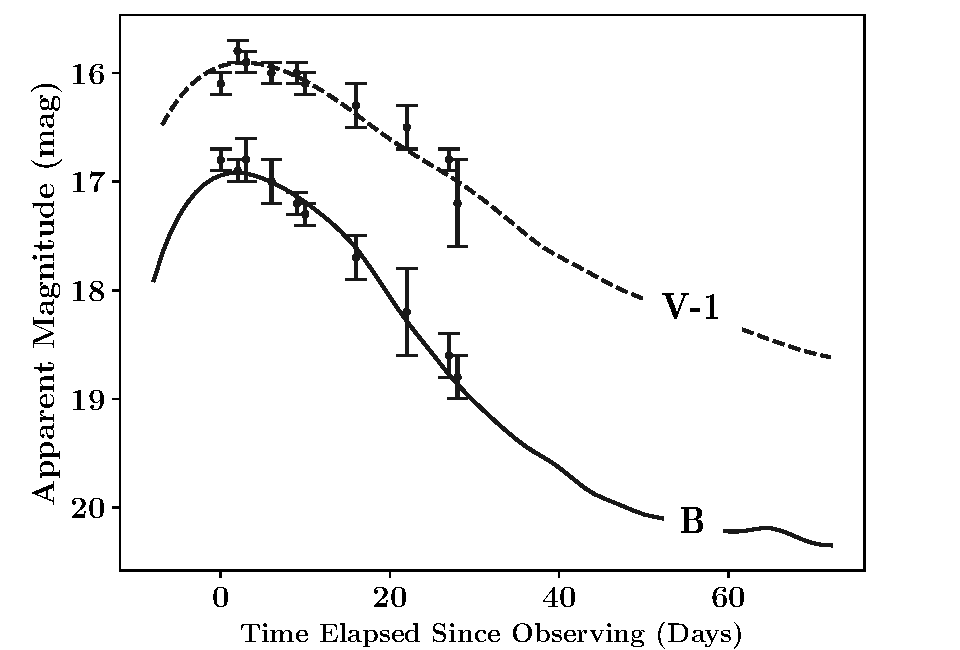
\includegraphics[width=9.5cm]{results/2017hhz}
\caption[]{Intensity maps of four different diffraction patterns taken from different planes: (a) double circle grating in Fourier plane, (b) single circle grating in Fourier plane, (c) L grating in image plane, (d) L grating in `$3f$' plane.}
\label{2017hhz-data}
\end{center}
\end{figure}

\vspace{-3ex}
\section{Discussion}
\label{discussion}
\vspace{-2ex}

It is highly unlikely that we will see supernova remnants for the supernova that we have been studying, in the shape of the Crab Nebula. Much longer time periods would be required for this. 

In observing objects which are so faint we have the problem of trying to observe them. We need to balance the observing time to ensure that we do not oversaturate our frame with other stars. From the databases that we use, for this observation period the majority of our objects had been around the magnitudes of $\sim 18$ mag. But, we do not achieve this magnitude as there are various factors such as extinction affectinb data collection. 

We can calculate the limitiing magnitude that our telescopes could detect by analysing our frames


[neutrino studying]?

SNooPy uses the Levenberg-Marquardt least-squares fitter to fit the model to the data [[cite]]. 

in using snoopy, how does it really fit the models to the data, what kind of parameters does it constrain. what is it's reliance on different parameters

try and produce some sort of covariance relation plot?

performing incorrect photometry and how that affects our results - not realising that we had to set a zero point, then having to find the zero point ourselves. 

confusion in observations, novae, cataclysmic variables 

there are other scripts which provide an automated way in finding the zero points from the data. what would this produce? why would this be beneficial to use this as opposed to our method?

justification of using the uncertainty equation, functional approach, why not use the uncertainty that was provided by the software? mention how it's one of the photon statistics things.

dstack, taking the median not mean , and why this is better - if I haven't discussed this already

what science have we addressed? well, we have limitations on the telescopes in terms of how 'deep' we can see:  the limiting magnitude, how that was calculated - longer exposure times...etc

has it been possible to plot a light curve with reasonable uncertainties? how best could this experiment be changed? 

big picture: justification of the uncertainties 

using the jackknife method to discover the range of uncertainties after we had used snoopy to fit a model, the whole different parameters relating to each other

covariance and correlations between parameters

statisitcal, experimental - different uncertainties

extinction and galaxy extinction taking them into calculations

hubble flow????

how does SNooPy actually work - maybe just give this a section

how using different fitting models to check the quality of the data, right now we haven't really explored the quality of our data. 




\vspace{-5ex}
\section{Conclusions}
\label{conclusions}
\vspace{-2ex}

sdfsdfasdas

\vspace{-5ex}
\section*{Acknowledgements}
\vspace{-2ex}
This research has made use of the CfA Supernova Archive, which is funded in part by the National Science Foundation through grant AST 0907903.


\bibliographystyle{abbrv}
\bibliography{supernovae}

\clearpage
\onecolumngrid
\vspace{-3ex}
\section*{Appendix A - Objects Log} \label{objectslog}
\vspace{-2ex}
A list of the objects that were chosen to be observed, and then the subsequent notes on them. Not all objects were chosen to be observed for an extended period, the ones noted were observed for a couple of nights to ensure suitability. The subsequent observation logs can be found in Appendix B.

{\renewcommand{\arraystretch}{1.2}%
\begin{table}[h!]
\centering    
\begin{tabularx}{\textwidth}{c c c c @{\hskip 5pt} c c X}
    \hline
    \textbf{Object} & \textbf{RA} & \textbf{Dec} & \textbf{Magnitude} &\textbf{First Discovered} &\textbf{Type} & \textbf{Notes} \\ 
    *ASASSN-17mz & 23:56:21.82 & +32:27:24.08 & 14.6 & 2017/09/30.500 & Ia & {Too close to galactic nucleus, cannot see}  \\
    *AT2017hld & 22:18:22.849 & +34:45:08.46 & 16.1 & 2017/10/17.339 & CV & {Cataclysmic Variable, stopped observing}  \\
    *2017hky & 11:23:30.514 & +63:21:59.43 & 16.2 & 2017/10/16.640 & II & {Not viewable from Durham or La Palma}  \\
    2017hhz & 01:44:16.75 & +12:15:18.00 & 16.83 & 2017/10/16.140 & Ia & {A measured redshift, $z=0.0392$}  \\
    AT2017gvb & 08:04:42.34 & +61:31:41.50 & 17.33 & 2017/09/26.59 & unk & {-}  \\
    *ASASSN-17nb & 07:27:37.32 & +35:36:28.30 & 17.31 & 2017/09/25.59 & II & {Object is dwarfed by brightness of the galaxy}  \\
    2017hle & 01:07:36.060 & +32:24:30.00 & 18.0 & 2017/10/18.684 & Ia-91bg & {-}  \\
    2017hou & 04:09:02.140 & -01:09:36.40 & 17.9 & 2017/10/24.370 &Ia & {Viewable from La Palma}  \\
    *AT2017hmw & 01:07:16.570 & +31:25:28.88 & 17.2 & 2017/10/19.415 & CV & {Cataclysmic Variable}  \\
    2017hpa & 04:39:50.750 & +07:03:54.90 & 17.9 & 2017/10/15.346 & Ia & {Viewable from La Palma}  \\
    *AT2017hnm & 01:42:03.24 & +42:31:08.50 & 16.69 & 2017/10/23.44 & unk & {Another star in the image dwarfs the SN in brightness}  \\
    AT2017hpm & 08:04:15.100 & -00:03:58.03 & 16.4 & 2017/10/26.290 & unk & {-}  \\
    *AT2017hqa & 01:08:59.160 & +32:38:04.10 & 17.3 & 2017/10/26.740 & unk & {Unobservable, too close to galactic centre}  \\
    2017hqc & 23:23:08.210 & +10:38:54.63 & 18.0 & 2017/10/27.490 & Ia & {-}  \\
    *AT2017hrr & 11:29:06.490 & -08:59:18.56 & 15.4 & 2017/10/30.607 & unk & {Cannot view from Durham or La Palma}  \\
    *AT2017hhq & 00:42:50.230 & +41:15:27.10 & 17.7 & 2017/10/30.599 & NV & {A nova close to M31}  \\
    AT2017htb & 22:09:38.520 & +17:39:39.56 & 15.7 & 2017/11/02.190 & unk & {-}  \\
    AT2017hzw & 02:05:18.337 & +53:12:13.16 & 17.3 & 2017/11/13.410 & Ia-CSM & {-}  \\
    2017igf & 11:42:49.850 & +77:22:12.94 & 15.4 & 2017/11/18.590 & Ia & {-}  \\
    \hline      
\end{tabularx}
\caption{Objects that we chose to observe and notes on them. RA is the Right Ascension, given in units of hours : arcminutes : arcseconds. Dec is the Declination, degrees : minutes : seconds. The stated magnitude is the initial magnitude that the object was discovered in the V band. Objects marked with an asterisk $*$ were objects which we chose to stop observing, the reason provided in the notes.}
\label{objects}
\end{table}


\clearpage

\onecolumngrid
\vspace{-3ex}
\section*{Appendix B - Observation Logs} \label{obslogs}
\vspace{-2ex}
Given below are all the observations which were made during our observation periods. The exposures column is of the following format: ($x: y, z$ s), where $x$ is the band in which the images were taken in, $y$ the number of exposures taken, and $z$ the exposure time which was used, in units of seconds.
{\renewcommand{\arraystretch}{1.2}%
\begin{table}[h!]
\centering    
\begin{tabularx}{\textwidth}{c@{\hskip 5pt} c c@{\hskip 5pt} c@{\hskip 5pt} c@{\hskip 5pt} X}
    \hline
    \textbf{Date} & \textbf{Object} & \textbf{Time} & \textbf{Exposures} & \textbf{  Conditions  } & \textbf{Notes} \\ 
    20/10/17 & 2017hhz & 22:25:34 to 22:58:50 & \makecell{B: 5, 120s \\ V: 5, 120s} & {Clear} & {pt5m: -}  \\
    	& ASASSN-17nb &  02:56:08 to 03:23:36 & \makecell{B: 5, 60s \\ V: 5, 60s} & {Cloudy} & {pt5m: Images produced have a lot of noise.} \\      
	
    21/10/17 & - & - & - & Cloudy & {\em No observations: weather not sufficient in Durham or La Palma for observations. \em} \\
    
    22/10/17 & AT2017hmw &  21:52:20 to 22:31:49 & \makecell{B: 5, 120s \\ V: 5, 120s} & {Clear} & {pt5m: -} \\  
    & 2017hhz & 22:40:20 to 23:19:50 & \makecell{B: 4, 60s \\ V: 12, 60s} & {Clear} & {pt5m: -}  \\
    & ASASSN-17nb &  02:42:45 to 03:10:46 & \makecell{B: 5, 120s \\ V: 5, 60s} & {Clear} & {pt5m: -} \\  
    & AT2017gvb & 03:12:31 to 03:58:58 & \makecell{B: 5, 180s \\ V: 5, 120s} & {Clear} & {pt5m: -} \\    
    
    23/10/17 & 2017hhz & 22:53:12 to 23:32:42 & \makecell{B: 5, 120s \\ V: 5, 120s} & {Cloudy} & {pt5m: Data produced has FWHM ranging from $1.6$ to $9.9$.} \\  
    
    24/10/17 & 2017hhz & 22:44:01 to 23:23:30 & \makecell{B: 5, 120s \\ V: 5, 120s} & {Cloudy} & {pt5m: Data is noisy, potentially another object transited across the frame while observing.} \\  
    
    25/10/17 & - & - & - & {Cloudy} & {\em No observations: too cloudy for observations in Durham, and items in pt5m queue were pushed out in favour of other objects. \em} \\
    
    26/10/17 & 2017hle & 20:54:44 to 21:09:03 & \makecell{B: 4, 60s \\ V: 4, 60s} & {Clear} & {FE16: - }  \\
    & 2017hhz &  21:18:00 to 21:25:31 & \makecell{B: 4, 60s \\ V: 4, 60s} & {Clear} & {FE16: -} \\ 
    & AT2017hmw &  21:29:15 to 21:39:36 & \makecell{B: 4, 60s \\ V: 4, 60s} & {Cloudy} & {FE16: -} \\
    & Messier-7 &  21:50:23 to 21:54:47 & {C: 1, 60s} & {Slightly Cloudy} & {FE16: Test object for SN discovery.} \\
    & Messier-10 &  21:55:47 to 22:00:13 & {C: 1, 60s} & {Cloudy} & {FE16: Test object for SN discovery.} \\
    & AT2017hnm &  23:27:22 to 23:41:55 & \makecell{B: 5, 120s \\ V: 3, 120s} & {Clear} & {pt5m: -} \\ 
    & AT2017gvb &  - & - & {-} & {pt5m: Object pushed out of the queue in favour of others.} \\

    27/10/17 & AT2017hqa & 18:48:12 to 18:52:59 & \makecell{B: 4, 60s} & {Cloudy} & {FE16: Object too close to galactic nucleus. }  \\
    & AT2017hnm &  18:56:34 to 19:00:23 & \makecell{C: 1, 60s} & {Slightly Cloudy} & {FE16: Object too dim, cloud cover reduced light we were receiving.} \\
    & Abell 426 &  19:04:23 to 19:15:41 & \makecell{C: 1, 60s \\ B: 9, 60s \\ V: 9, 60s} & {Clear} & {E14: Object to observe to discover new SN.} \\
    & 2017hhz &  20:11:35 to 20:22:43 & \makecell{B: 4, 60s \\ V: 4, 60s} & {Cloudy and Windy} & {E14: Seeing is bad due to the weather.} \\
    & 2017hle &  20:26:18 to 20:37:35 & \makecell{B: 4, 90s \\ V: 4, 90s} & {Slightly Cloudy} & {E14: Seeing is bad in these images as well.} \\
    & 2017hou &  23:48:09 to 23:50:14 & \makecell{B: 2, 120s} & {-} & {pt5m: Only two frames taken, not sufficient data.} \\
    \hline      
\end{tabularx}
\label{obs_logs1}
\end{table}

{\renewcommand{\arraystretch}{1.2}%
\begin{table}[h!]
\centering    
\begin{tabularx}{\textwidth}{c@{\hskip 5pt} c c@{\hskip 5pt} c@{\hskip 5pt} c@{\hskip 5pt} X}
    \hline
    \textbf{Date} & \textbf{Object} & \textbf{Time} & \textbf{Exposures} & \textbf{  Conditions  } & \textbf{Notes} \\ 
    27/10/17 & AT2017gvb &  02:16:01 to 03:03:05 & \makecell{B: 5, 120s \\ V: 5, 120s} & {Clear/Cloudy} & {pt5m: Some images are more noisy due to clouds.} \\
    
    28/10/17 & AT2017hnm &  21:41:55 to 22:21:25 & \makecell{B: 5, 120s \\ V: 5, 120s} & {Clear} & {pt5m: -} \\
    & 2017hhz &  21:28:50 to 21:30:50 & \makecell{B: 1, 120s} & {Clear} & {pt5m: -} \\
    
    29/10/17 & 2017hle &  21:22:39 to 21:41:21 & \makecell{B: 10, 120s \\ V: 1, 120s} & {Clear} & {pt5m: Mistake on our part to take so many images in B band, and only one in V band.} \\
    & AT2017hnm &  21:55:34 to 22:35:04 & \makecell{B: 5, 120s \\ V: 5, 120s} & {Slightly Cloudy} & {pt5m: -} \\
    & 2017hhz &  23:16:48 to 23:56:18 & \makecell{B: 5, 120s \\ V: 5, 120s} & {Clear} & {pt5m: -} \\
    & 2017hou &  00:33:33 to 01:13:02 & \makecell{B: 5, 120s \\ V: 5, 120s} & {Clear} & {pt5m: -} \\
    & 2017hqc &  01:16:20 to 01:41:20 & \makecell{B: 4, 120s \\ V: 4, 120s} & {Clear} & {pt5m: -} \\
    & AT2017gvb &  02:18:51 to 02:55:47 & \makecell{V: 13, 180s} & {Clear} & {pt5m: Long exposure and large number of exposures chosen as a test to see the quality of stacking them.} \\
    
    30/10/17 & 2017hle &  21:18:56 to 21:58:25 & \makecell{B: 10, 120s \\ V: 10, 120s} & {Clear} & {pt5m: -} \\
    & 2017hhz &  22:06:34 to 22:46:04 & \makecell{B: 5, 120s \\ V: 5, 120s} & {Clear} & {pt5m: -} \\
    & AT2017gvb &  02:04:22 to 03:02:50 & \makecell{V: 20, 180s} & {Clear} & {pt5m: An human error, we re-selected this object from the previous night instead of the one with the correct number of required frames for each band.} \\
    
    31/10/17 & - & - & - & {Cloudy} & {\em No observations: too cloudy for observations in Durham and La Palma. \em} \\
    
    01/11/17 & 2017hle & 23:56:53 to 00:15:35 & \makecell{B: 5, 120s \\ V: 5, 120s} & Clear & {pt5m: -} \\
    & AT2017hnm & 00:18:23 to 00:57:55 & \makecell{B: 5, 120s \\ V: 5, 120s} & Clear & {pt5m: -} \\
    & 2017hhz & 01:00:47 to 01:40:17 & \makecell{B: 5, 120s \\ V: 5, 120s} & Clear & {pt5m: -} \\
    & 2017hou & 01:43:38 to 02:23:08 & \makecell{B: 5, 120s \\ V: 5, 120s} & Clear & {pt5m: -} \\
    
    02/11/17 & - & - & - & {Cloudy} & {\em No observations: too cloudy for observations in Durham and La Palma. \em} \\
    
    03/11/17 & - & - & - & {Cloudy} & {\em No observations: too cloudy for observations in Durham and La Palma. \em} \\
    
    04/11/17 & - & - & - & {Cloudy} & {\em No observations: too cloudy for observations in Durham and La Palma. \em} \\
    
   05/11/17 & ASASSN-17mz & 17:53:45 to 18:09:34 & \makecell{B: 8, 60s \\ V: 8, 60s} & {Clear} & {FE16: -} \\
   & 2017hhz & 18:50:39 to 19:24:43 & \makecell{B: 8, 120s \\ V: 8, 60s} & {Clear} & {FE16: -} \\
   & AT2017htb & 19:38:14 to 20:02:16 & \makecell{B: 8, 60s \\ V: 8, 60s} & {Slightly Cloudy} & {W14: -} \\
   & 2017hle & 20:05:49 to 20:08:28 & \makecell{V: 2, 60s} & {Cloudy} & {W14: Stopped taking exposures after viewing the weather.} \\
   & 2017hqc & 20:14:16 to 20:18:25 & \makecell{V: 3, 60s} & {Cloudy} & {W14: Seeing if images will be strongly affected by the cloud cover.} \\
   & AT2017hhq & 20:33:58 to 20:42:26 & \makecell{B: 4, 60s \\ V: 4, 60s} & {Clear} & {W14: -} \\
       \hline      
\end{tabularx}
\label{obs_logs2}
\end{table}

{\renewcommand{\arraystretch}{1.2}%
\begin{table}[h!]
\centering    
\begin{tabularx}{\textwidth}{c@{\hskip 5pt} c c@{\hskip 5pt} c@{\hskip 5pt} c@{\hskip 5pt} X}
    \hline
    \textbf{Date} & \textbf{Object} & \textbf{Time} & \textbf{Exposures} & \textbf{  Conditions  } & \textbf{Notes} \\ 
    05/11/17 & AT2017hhq & 19:38:14 to 20:02:16 & \makecell{B: 3, 30s \\ V: 3, 30s \\ R: 3, 30s} & {Cloudy} & {E14: Images taken so that we can produce a colour image. } \\
    
    06/11/17 & - & - & - & {Cloudy, and Rain} & {\em No observations: too cloudy for observations in Durham, and torrential rain in La Palma. \em} \\
    
    07/11/17 & - & - & - & {Cloudy and Rain} & {\em No observations: too cloudy for observations in Durham, and torrential rain in La Palma. \em} \\
    
    08/11/17 & - & - & - & {Cloudy and Rain} & {\em No observations: too cloudy for observations in Durham, and torrential rain in La Palma. \em} \\
    
    09/11/17 & - & - & - & {Cloudy and Rain} & {\em No observations: too cloudy for observations in Durham, La Palma was not functioning. \em} \\
    
    10/11/17 & 2017hhz & 19:15:32 to 19:31:57 & \makecell{B: 4, 90s \\ V: 2, 90s} & {Cloudy} & {FE16: -} \\
    & 2017hqc & 19:37:27 to 19:49:15 & \makecell{B: 4, 90s \\ V: 2, 90s} & {Cloudy} & {FE16: -} \\
    
    11/11/17 & 2017hhz & 19:15:32 to 19:31:57 & \makecell{B: 4, 90s \\ V: 2, 90s} & {Cloudy} & {FE16: -} \\
    
       \hline      
\end{tabularx}
\caption{Observing logs for the entire observation period for our experiment.}
\label{obs_logs3}
\end{table}


\clearpage

\twocolumngrid
\vspace{-3ex}
\section*{Appendix C - Set of Sample Data}
\vspace{-2ex}

asdasda

\clearpage

\twocolumngrid
\vspace{-3ex}
\section*{Appendix D - Uncertainties}
\vspace{-2ex}

\end{document}
